% Suggested figure blocks; integrate only after final complete-ensemble reductions.
\begin{figure*}
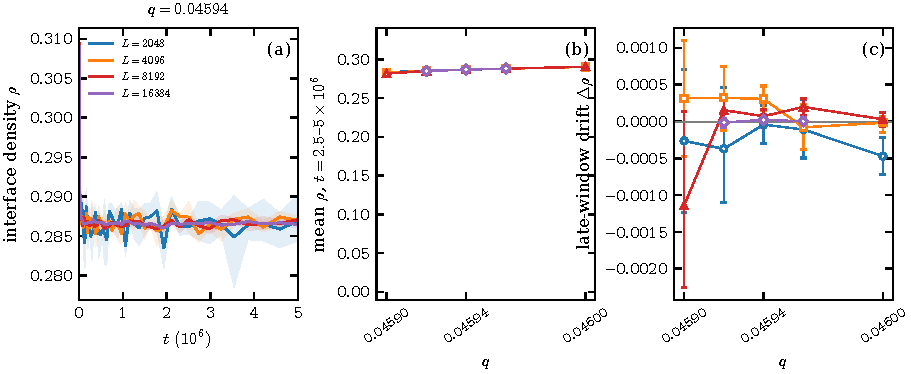
\includegraphics[width=\textwidth]{figs/fig_gpu_bulk}
\caption{Long, large-system bulk tests at $p=\alpha=1/2$, with four independent
random starts per $(L,q)$ and $T=5\times10^6$.
(a) Interface density at $q=0.04594$; bands are pointwise 95\% run-bootstrap
intervals. (b) Unconditional time-weighted density over
$2.5\times10^6\le t\le5\times10^6$ against the actual probability $q$.
(c) Difference between means over $3.75$--$5\times10^6$ and
$2.5$--$3.75\times10^6$; zero indicates no resolved drift between these
windows. Error bars in (b,c) are 95\% run-bootstrap intervals.
Every declared seed contributes; absorbed trajectories contribute their known
absorbing state for the rest of the observation window.}
\label{fig:gpu_bulk}
\end{figure*}

\begin{figure*}
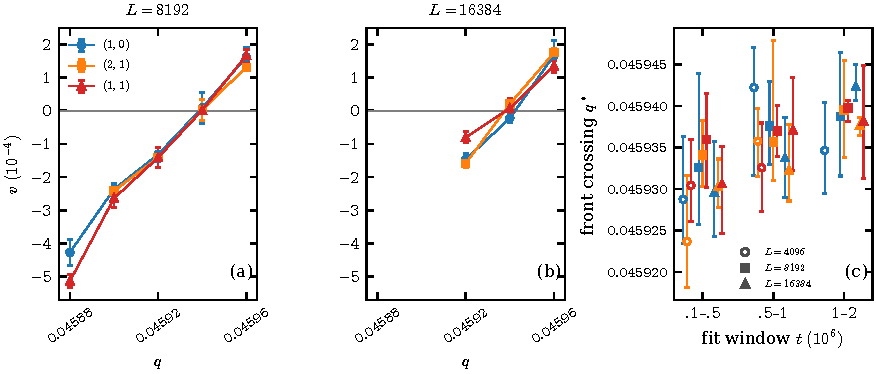
\includegraphics[width=\textwidth]{figs/fig_gpu_fronts}
\caption{Fine-grid front measurements at $p=\alpha=1/2$.
(a,b) Normal velocities at $L=8192$ and $16384$, fitted over
$10^6\le t\le2\times10^6$; four independent bands per point, and bars are
one standard error over runs. Colors and markers distinguish the three band
normals. Each included group retains a separated pair of fronts throughout
the stated fit window in every run.
(c) Local bracketing estimates of the velocity zero for three successive
windows; colors denote the same normals, while marker shapes denote $L$.
The $L=4096$ groups have eight runs, and the larger sizes four.
Intervals are conditional 95\% run-bootstrap intervals for each chosen
window and threshold. The variation between windows and orientations is
shown separately from sampling uncertainty.}
\label{fig:gpu_fronts}
\end{figure*}

\begin{figure*}
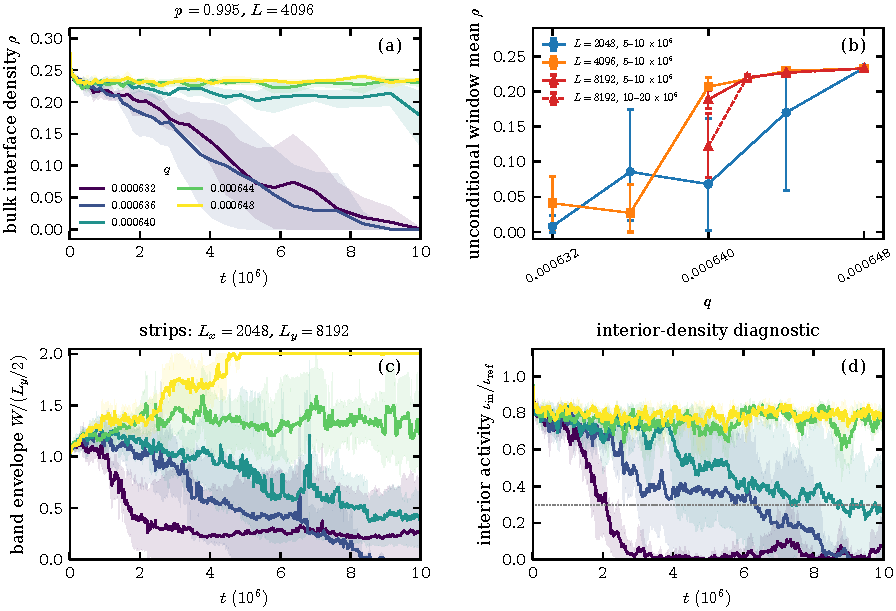
\includegraphics[width=\textwidth]{figs/fig_gpu_near}
\caption{Long-time tests near the voter point, $p=0.995$, $\alpha=1/2$;
four independent runs per parameter set. Colors in (a,c,d) denote the same $q$.
(a) Bulk density at $L=4096$ to $10^7$ steps.
(b) Unconditional time-weighted bulk means over a common
$5\times10^6\le t\le10^7$ window at three sizes, together with the later
$10^7$--$2\times10^7$ window at $L=8192$.
(c) Outer-envelope width of initially half-filled active strips,
$L_x=2048$, $L_y=8192$, normalized by the initial half-box width.
(d) Activity in the initial central interior region, relative to its
reference value at $t=10^3$. The dotted line is the profile threshold used
for the envelope. A changing interior density must be distinguished from
motion of a stationary front. Bands and bars are pointwise 95\%
run-bootstrap intervals. Absorbed trajectories are extended by their known
zero activity, and only complete predeclared seed ensembles are shown.}
\label{fig:gpu_near}
\end{figure*}

\begin{figure*}
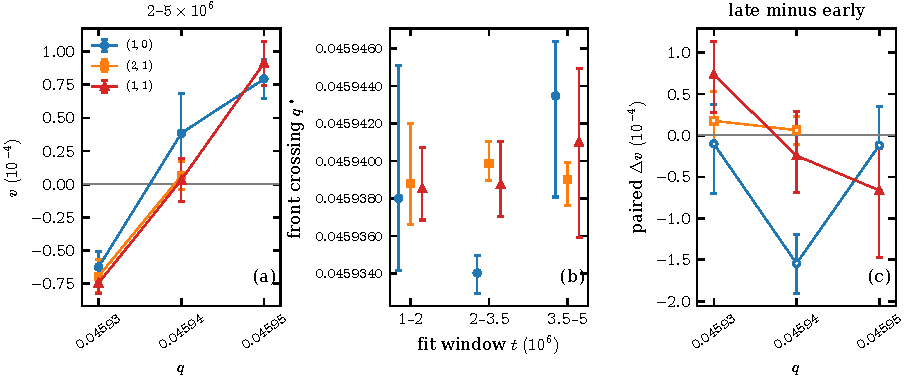
\includegraphics[width=\textwidth]{figs/fig_gpu_fronts5m}
\caption{Independent long-time front-stationarity test at $p=\alpha=1/2$,
$L=8192$, with four new seeds per $(q,\mathrm{normal})$ and $T=5\times10^6$.
These cohorts are separate from the original $T=2\times10^6$ cohorts.
(a) Normal velocities fitted over $2$--$5\times10^6$, with one standard
error over runs. (b) Local bracketing crossings in successive windows
within the new cohorts, with conditional 95\% run-bootstrap intervals.
(c) Paired differences $v_{3.5\text{--}5\times10^6}-v_{2\text{--}3.5\times10^6}$;
each difference uses the same run in both windows, and bars are 95\%
run-bootstrap intervals. Only complete predeclared four-seed groups with
valid separated-front geometry throughout both windows contribute.
Crossings are shown only when bracketed within the declared $q$ grid;
unbracketed windows are not extrapolated. Threshold and interpolation choices
remain separate systematic uncertainties. A nonzero paired difference records
temporal drift; a zero-containing interval alone does not establish stationarity.}
\label{fig:gpu_fronts5m}
\end{figure*}
